\documentclass[10pt, aspectratio=169]{beamer}

\usetheme[progressbar=frametitle]{metropolis}
\usepackage{appendixnumberbeamer}

\usepackage{booktabs}
\usepackage[scale=2]{ccicons}

\usepackage{pgfplots}
\usepgfplotslibrary{dateplot}

\usepackage{xspace}
\newcommand{\themename}{\textbf{\textsc{metropolis}}\xspace}
\usepackage[utf8]{inputenc}

%\setbeamercovered{transparent}

\title{Preparazione di polvere di biopolimeri}
\subtitle{Stampa 3D tramite Selective Laser Sintering}
% \date{\today}
\date{}
\author{Giorgio De Trane}
\institute{Politecnico di Torino}
\titlegraphic{\hfill
\includegraphics[height=1.5cm]{Pictures/Vector/PDF/polito_logo.pdf}}

\begin{document}

\maketitle

\begin{frame}{Contenuti}
  \setbeamertemplate{section in toc}[sections numbered]
  \tableofcontents[hideallsubsections]
\end{frame}


\section{Introduzione}
  \subsection{Obiettivo}

  \begin{frame}{Obiettivo}
    
    \begin{itemize}
      \item <1->\textbf{Preparazione} di polvere di biopolimeri
      \item <2>\textbf{Stampa 3D} di biopolimeri
    \end{itemize}
  \end{frame}

  \begin{frame}
    \frametitle{Biopolimeri}
    \begin{center}
        Perchè \textbf{biopolimeri}?
    \end{center}
    \begin{figure}[h]
      \centering
      \includegraphics[width=0.3\textwidth]{Pictures/Vector/PDF/hand_bio.pdf}
      
    \end{figure}

  \end{frame}

  \begin{frame}
    \frametitle{Perchè biopolimeri?}
    \begin{itemize}
      \item <1->\textbf{Biodegradabili}
      \item <2->\textbf{Biocompatibili}
      \item <3->\textbf{Riciclabili}
      \item <4> \textbf{Sostenibili}
    \end{itemize}


  \end{frame}
    
  
  
  \subsection{Ricerca}

  \begin{frame}{Ricerca}
    \begin{itemize}
      \item <1-> Stato dell'arte dei \textbf{polimeri} nella \textbf{stampa 3D}
      \item <2->  \textbf{Biopolimeri} nella \textbf{stampa 3D}
      \item <3->  Produzione di \textbf{polvere} per \textbf{Selective Laser Sintering}
    \end{itemize}

    \onslide<4>{\alert<4>{Pochissimi} risultati in letteratura!}

  \end{frame}

  \begin{frame}
    \frametitle{Selective Laser Sintering}
  
    \onslide*<1>{La Sinterizzazione Selettiva con laser o \textbf{SLS} 
    è una tecnologia di produzione additiva che impiega un raggio laser per sinterizzare delle particelle 
    di polvere che può essere a base polimerica o composita}

    %\onslide*<2>{
    %\begin{figure}[h]
    %  \centering
    %  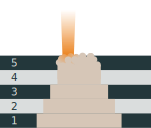
\includegraphics[width=0.5\textwidth]{Pictures/Vector/PDF/SLS_scheme.pdf}
    %\end{figure}
    %}
  
  \end{frame}
  \subsection{Scelta del biopolimero}
  \begin{frame}{Scelta del biopolimero}
    \onslide*<1>{
      \begin{center}
        Finestra di \textbf{sinterizzazione}
      \end{center}
    }
    \onslide*<2>{Finestra di sinterizzazione}

    \onslide*<2>{
      \begin{center}
        Range di temperatura tra la \textbf{cristallizzazione} e la \textbf{fusione} del polimero
      \end{center}
    }

    \onslide*<3>{
      \begin{center}
        \textbf{PHBH} \\ 
        Polyhydroxybutyratehexanoate
      \end{center}
    }

    \only<3>{
      \begin{figure}[h]
        \centering
        \includegraphics[width=0.5\textwidth]{Pictures/Vector/PDF/phbh_molecule.pdf}
        
      \end{figure}
    }
  \end{frame}
\section{Produzione della polvere}
  \section{Caratterizzazione della polvere}
    \subsection{Microscopia a Scansione Elettronica}
    \subsection{Distribuzione granulometrica}
    \subsection{Analisi termogravimetrica}
    \subsection{Analisi termica differenziale}
\section{Stampa 3D}
\section{Conclusioni}










\end{document}